%----------------------------------------------------------------------
% Problem 1

\begingroup
\allowdisplaybreaks

\newpage
\section{Problem 1}

\subsection{Solution}

\subsubsection{Part A}

The \verb|landweber()| function was implemented in \MATLAB, and a screenshot of the code is provided in figure \ref{fig: prob1 landweber}.

\begin{figure}[h] 
	\centering
	\includegraphics[width=0.625\textwidth]{./images/landweber.png}
	\caption{\MATLAB Landweber Function Screenshot}
	\label{fig: prob1 landweber}
\end{figure}
\FloatBarrier

\subsubsection{Part B}

\MATLAB code was modified from \verb|ex_6_2.m| to load image data, apply noise, and plot the resulting images. The fixed step size 

\begin{align*}
	\omega = 0.95 \frac{2}{s_1^2} = 6190.5
\end{align*}

was computed using the \verb|svds()| function in \MATLAB. A total of 500 iterations were running using the \verb|landweber()| function shown in figure \ref{fig: prob1 landweber}. Iterations 10, 50, 100, 150, 250, and 500 are evaluated. 

\begin{figure}[h] 
	\centering
	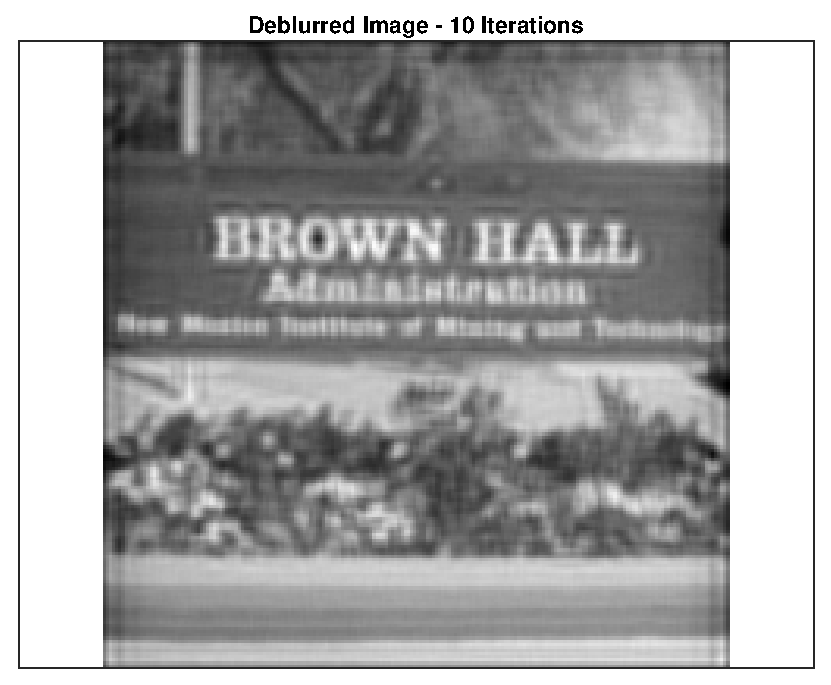
\includegraphics[width=0.5\textwidth]{./images/prob1_deblurred_image_10_iterations.eps}
	\caption{Deblurred Image - 10 Iterations}
	\label{fig: prob1 10 iterations}
\end{figure}
\FloatBarrier

\begin{figure}[h] 
	\centering
	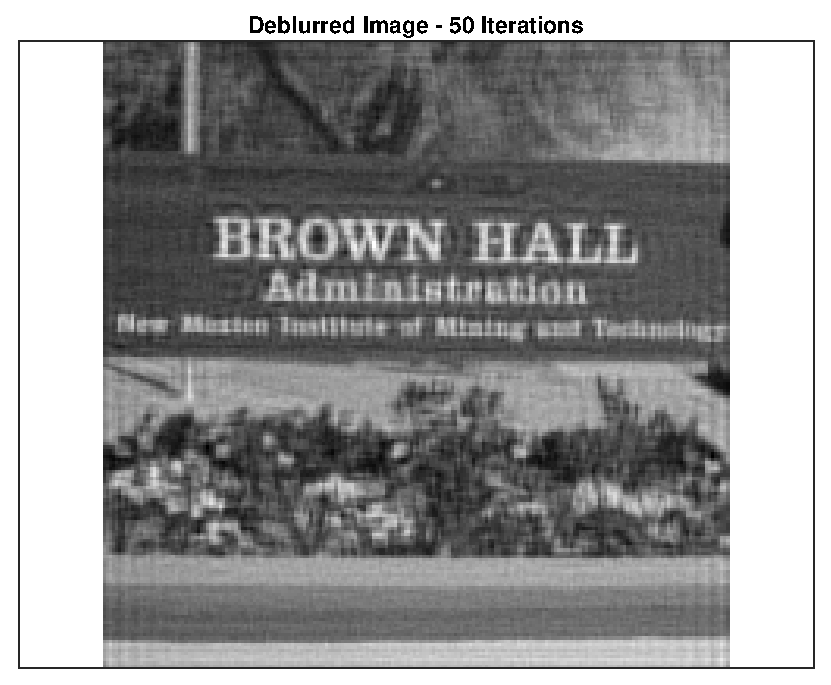
\includegraphics[width=0.5\textwidth]{./images/prob1_deblurred_image_50_iterations.eps}
	\caption{Deblurred Image - 50 Iterations}
	\label{fig: prob1 50 iterations}
\end{figure}
\FloatBarrier

\begin{figure}[h] 
	\centering
	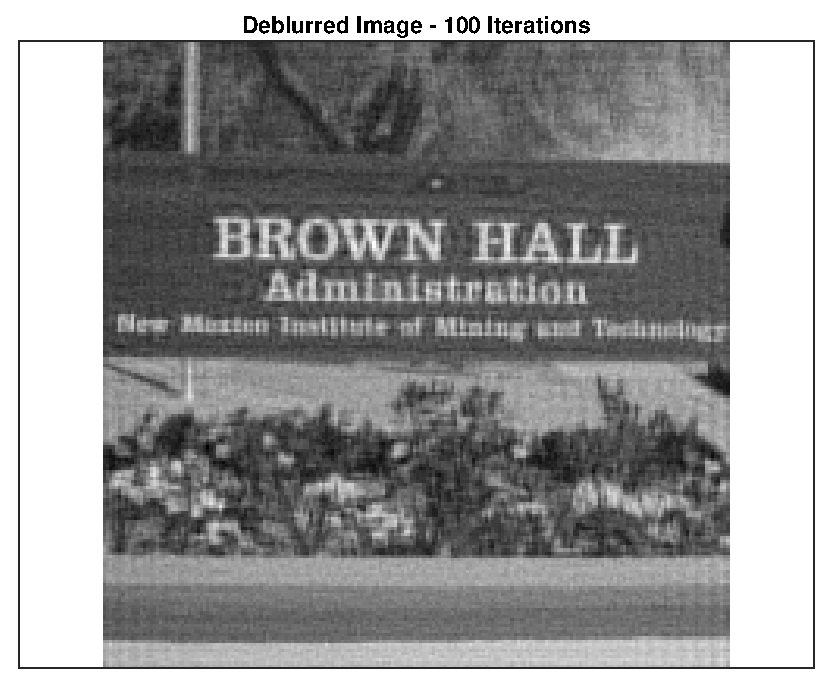
\includegraphics[width=0.5\textwidth]{./images/prob1_deblurred_image_100_iterations.eps}
	\caption{Deblurred Image - 100 Iterations}
	\label{fig: prob1 100 iterations}
\end{figure}
\FloatBarrier

\begin{figure}[h] 
	\centering
	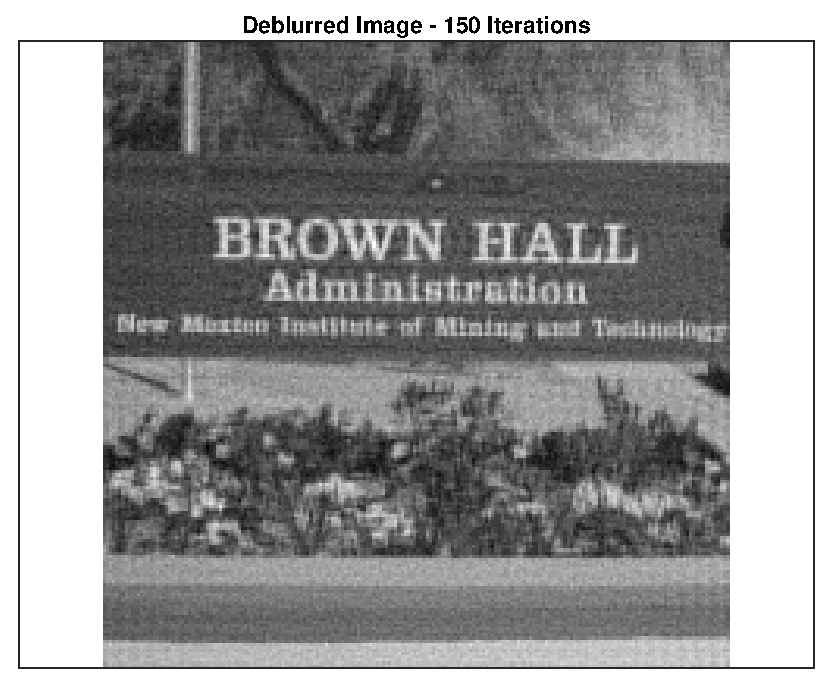
\includegraphics[width=0.5\textwidth]{./images/prob1_deblurred_image_150_iterations.eps}
	\caption{Deblurred Image - 150 Iterations}
	\label{fig: prob1 150 iterations}
\end{figure}
\FloatBarrier

\begin{figure}[h] 
	\centering
	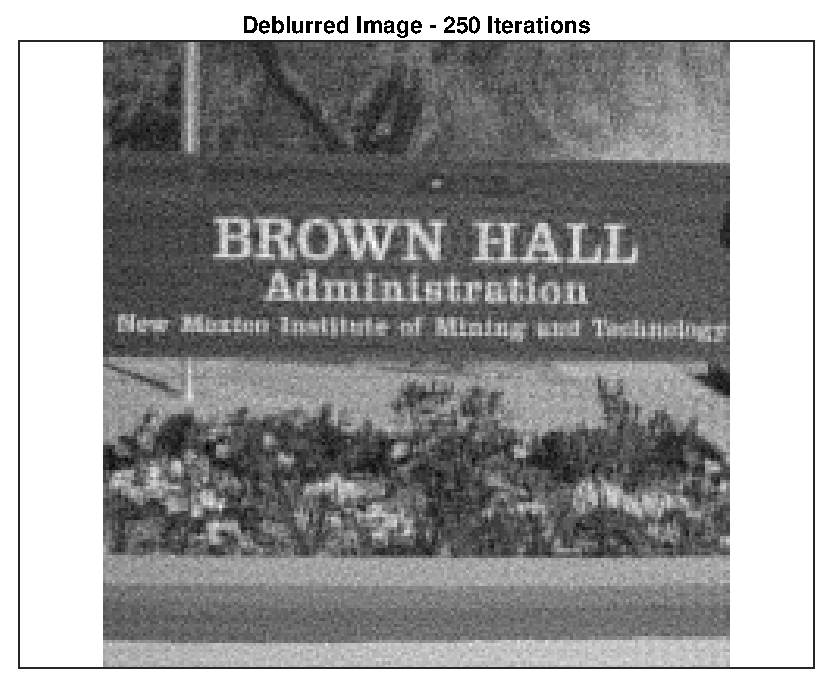
\includegraphics[width=0.5\textwidth]{./images/prob1_deblurred_image_250_iterations.eps}
	\caption{Deblurred Image - 250 Iterations}
	\label{fig: prob1 250 iterations}
\end{figure}
\FloatBarrier

\begin{figure}[h] 
	\centering
	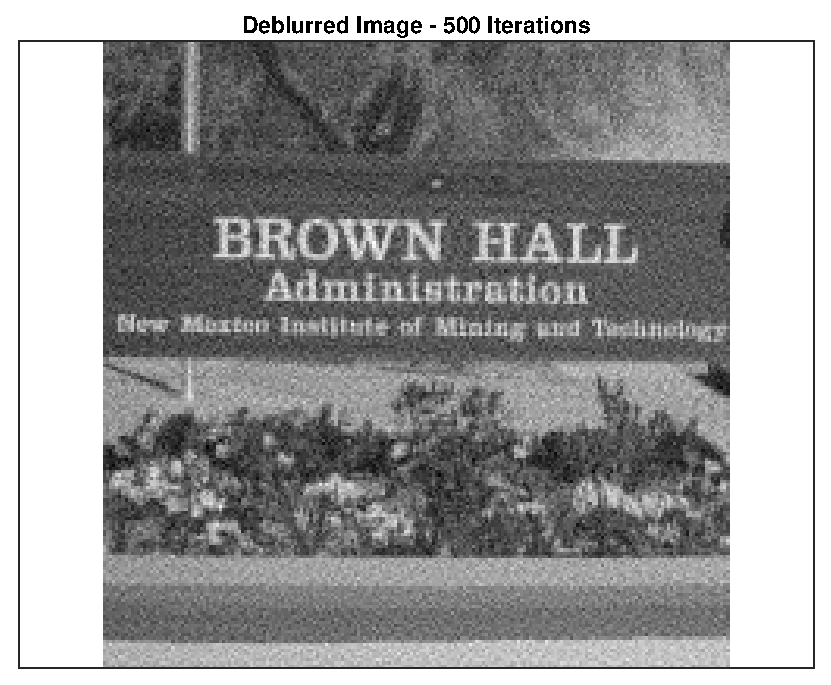
\includegraphics[width=0.5\textwidth]{./images/prob1_deblurred_image_500_iterations.eps}
	\caption{Deblurred Image - 500 Iterations}
	\label{fig: prob1 500 iterations}
\end{figure}
\FloatBarrier

It becomes clear that there is a "diminishing rate of returns" on the number of iterations used to deblur the image. In my opinion, it seems that the sharpest image appears at 150 iterations. The images after this number of iterations are also as sharp, but from there I can no longer tell a difference. 

It is less clear in this PDF, but on my screen in MATLAB it shows just a bit clearer. Unfortunately, you'll just have to take my word for it.


